% This is LLNCS.DEM the demonstration file of
% the LaTeX macro package from Springer-Verlag
\documentclass[a4paper,12pt]{llncs}
%
\usepackage{makeidx}  % allows for indexgeneration
\makeindex

\usepackage[ngerman]{babel}
\usepackage[utf8]{inputenc}      % Code-Page latin 1
\usepackage[T1]{fontenc}
% Nur eine der beiden folgenden Zeilen einbinden!
% siehe Abschnitt Bilder
%\usepackage{graphicx}       % Bilder einbinden, Version fuer normales latex
\usepackage[pdftex]{graphicx}       % Bilder einbinden, Version fuer pdflatex

% mit Hyperrefs
\usepackage[pdftex, plainpages=false,hypertexnames=true,pdfnewwindow=true,backref=true,colorlinks=true,citecolor=blue,linkcolor=black,urlcolor=blue,filecolor=blue]{hyperref}% 
% weitere Packages
\usepackage{ifthen}                 % Zum Auskommentieren von Textteilen
\usepackage{amssymb}                % Mathematische Buchstaben
\usepackage{amsmath}                % Verbesserter Formelsatz
\usepackage[vlined,boxed]{algorithm2e}
\usepackage{booktabs}               % schönere Tabellen
\usepackage{color}
\usepackage{hyperref}
 \hypersetup{urlcolor=black,citecolor=black}
%\setalcapskip{1.5ex} % fuer package algorithm
\usepackage{dsfont}  
%\newtheorem{definition}{Definition}
\usepackage{doc}
\usepackage{listings}
\usepackage{subcaption}
\usepackage{url}

% Seitenformat ===============================================================
\hoffset=-1.25truecm
\setlength{\topmargin}{0.0cm}
\setlength{\textheight}{23.0cm}
\setlength{\footskip}{1.5cm}
\setlength{\textwidth}{15.4cm}
\setlength{\evensidemargin}{1.5cm}
\setlength{\oddsidemargin}{1.5cm}
\setlength{\parskip}{1ex}
\setlength{\parindent}{0pt}
\setlength{\marginparwidth}{1.4cm}
\setlength{\marginparsep}{1mm}
\setalcapskip{1.5ex} % fuer package algorithm

\pagestyle{plain}

% Makro-Definitionen ==========================================================
% Zahlenbereiche -------------------------------------------------------------
\newcommand{\N}{{\mathbb{N}}}
\newcommand{\R}{{\mathbb{R}}}
\newcommand{\C}{{\mathbb{C}}}
\newcommand{\Z}{{\mathbb{Z}}}
\newcommand{\Q}{{\mathbb{Q}}}

% 
\def\myverzeichnis{.}

\numberwithin{equation}{section} 
% Bild -----------------------------------------------------------------------
% #1 Filename;  #2 Label;  #3 Bildunterschrift;  #4 Kurzform
\newcommand{\bild}[4]{
  \begin{figure}[htbp]
    \begin{center}
      \includegraphics{#1}
      \caption[#4]{#3}
      \label{#2}
    \end{center}
  \end{figure}
}

% Bildbreite -----------------------------------------------------------------
% #1 Filename;  #2 Breite;  #3 Label;  #4 Bildunterschrift;  #5 Kurzform
\newcommand{\bildbreite}[5]{
  \begin{figure}[htbp]
    \begin{center}
      \includegraphics[width=#2]{#1}
      \caption[#5]{#4}
      \label{#3}
    \end{center}
  \end{figure}
}

% !TeX spellcheck = de_DE
% ============================================================================
\begin{document}

% =========== Das war der Vorspann, jetzt geht's los! ========================

% ============================================================================
% =============  AB HIER DARF UND SOLL GETIPPT WERDEN ========================
% ============================================================================

\author{Yaroslav Nalivayko}
\index{Yaroslav Nalivayko}

% Das Institut wird fuer den Betreuer missbraucht ...
\institute{{\bf Betreuer:} M.Sc. Benjamin Maier}
\authorrunning{Yaroslav Nalivayko}
\title{Newton Fraktale}

\maketitle

\thispagestyle{empty}

\begin{abstract}
Newton Fraktale sind die Teilmenge der mathematischen Fraktale, die durch die Einsetzung des Newton Verfahrens für die Lösung der nichtlinearen Gleichungen auf der komplexe Ebene erscheinen.
\end{abstract}

% Einleitung -----------------------------------------------------------------
\section{Einleitung}
Newton Fraktale stellen eine interessante Klasse der mathematischen Fraktalen dar. 
Im Rahmen dieser Arbeit werden \nameref{sec:theo} vorgestellt und ein Programm für die \nameref{sec:vis} der Fraktalen entwickelt. In der letzten Sektion findet die \nameref{sec:analy} mancher interessanten Funktionen statt.


\section{Theoretische Grundlagen}\label{sec:theo}
Hier werden wichtigste Grundbegriffe erläutert.

\subsection{Numerische Mathematik}
Die numerische Mathematik beschäftigt sich als Teilgebiet der Mathematik mit der Konstruktion und Analyse von Algorithmen für kontinuierliche mathematische Probleme.~\cite{nummath}
Sie wird oft benutzt, um approximative Lösungen mit Hilfe des Rechners zu finden.

\subsection{Newton Verfahren}
Newton Verfahren ist das iterative numerische Verfahren, das die Wurzel gegebener Funktion findet.
Die Methode ist nach Sir Isaac Newton benannt. \\
Wir interessieren uns in stetig differenzierbaren Funktionen mit nur eine Variable.
\[
f(x) = 0
\] 
Man wählt den Startwert $x_0$ manuell und benutzt die iterative Methode, soweit eine akzeptable Lösung gefunden wird.
\[
x_{n+1} = x_n + \frac{f(x_n)}{f'(x_n)}
\] 
Gewöhnlich wählt man eine zulässige Abweichung $\varepsilon$ und eine maximale Anzahl der Schritte $N$.
Nach jedem Schritt der iterative Methode prüft man, ob $f(x_n)  < \varepsilon$ ist. 
In diesem Fall ist die Lösung gefunden.
Und falls $n > N$, dann ist die Lösung unauffindbar in die akzeptable Anzahl der Schritte. 
Iterative Prozess der Annäherung von $x_n$ zu $x_n+1$ heißt die Konvergenz, und falls $x_0$ zu $x_n$ kommt, heißt das, dass $x_0$ gegen $x_n$ konvergiert.

\subsection{Fraktale}
Fraktal (lateinisch $fractus$ - gebrochen) ist ein von Mathematiker Benoît Mandelbrot geprägter Begriff, der bestimmte natürliche oder künstliche Gebilde oder Muster bezeichnet. 
Diese Gebilde oder Muster weisen einen hohen Grad von Skaleninvarianz bzw. Selbstähnlichkeit. 
Das ist beispielsweise der Fall, wenn ein Objekt aus mehreren verkleinerten Kopien seiner selbst besteht.~\cite{fraktal} \\
Die Figur \ref{fig:frac_kunst} stellt ein Beispiel für ein künstliches Fraktal, und die Figur~\ref{fig:frac_math} für ein mathematisches Fraktal.
\begin{figure}[ht]   
	\begin{subfigure}{.5\textwidth}
	\centering
	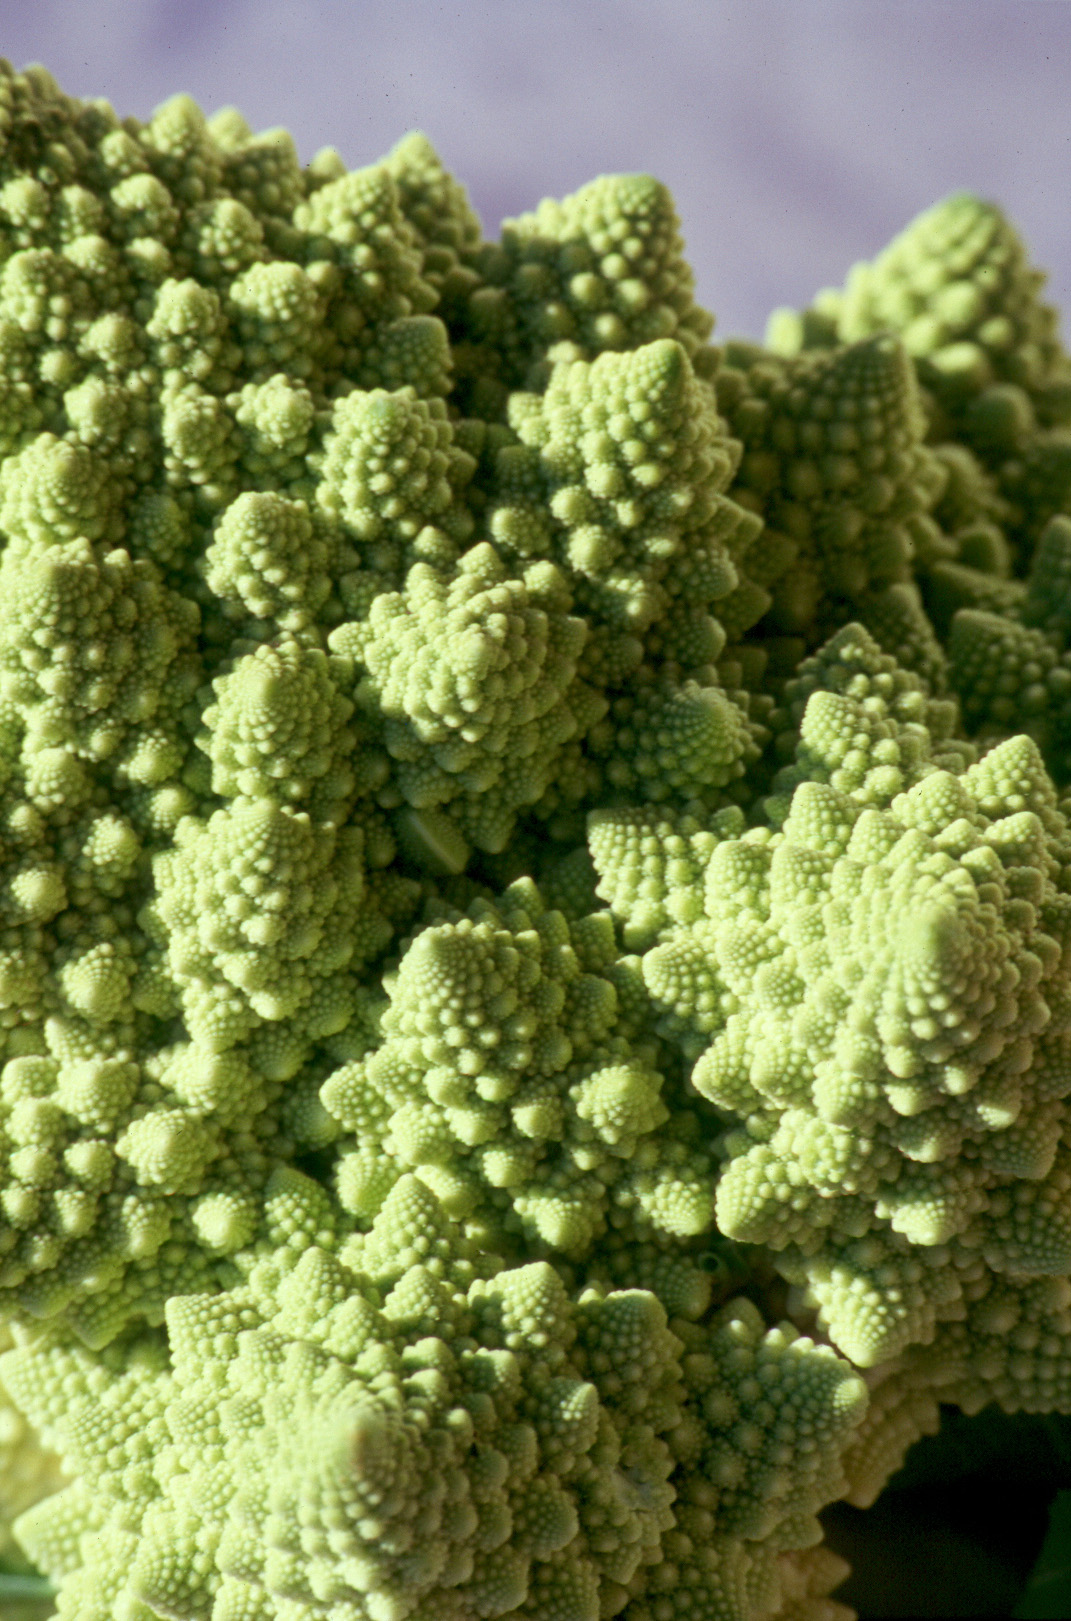
\includegraphics[width=.6\linewidth]{figures/Romanesco}
	\caption{Romanesco. Ein natürliches Fraktal.~\cite{fractal_romanesco}}
	\label{fig:frac_kunst}
\end{subfigure}%
\begin{subfigure}{.5\textwidth}
	\centering
	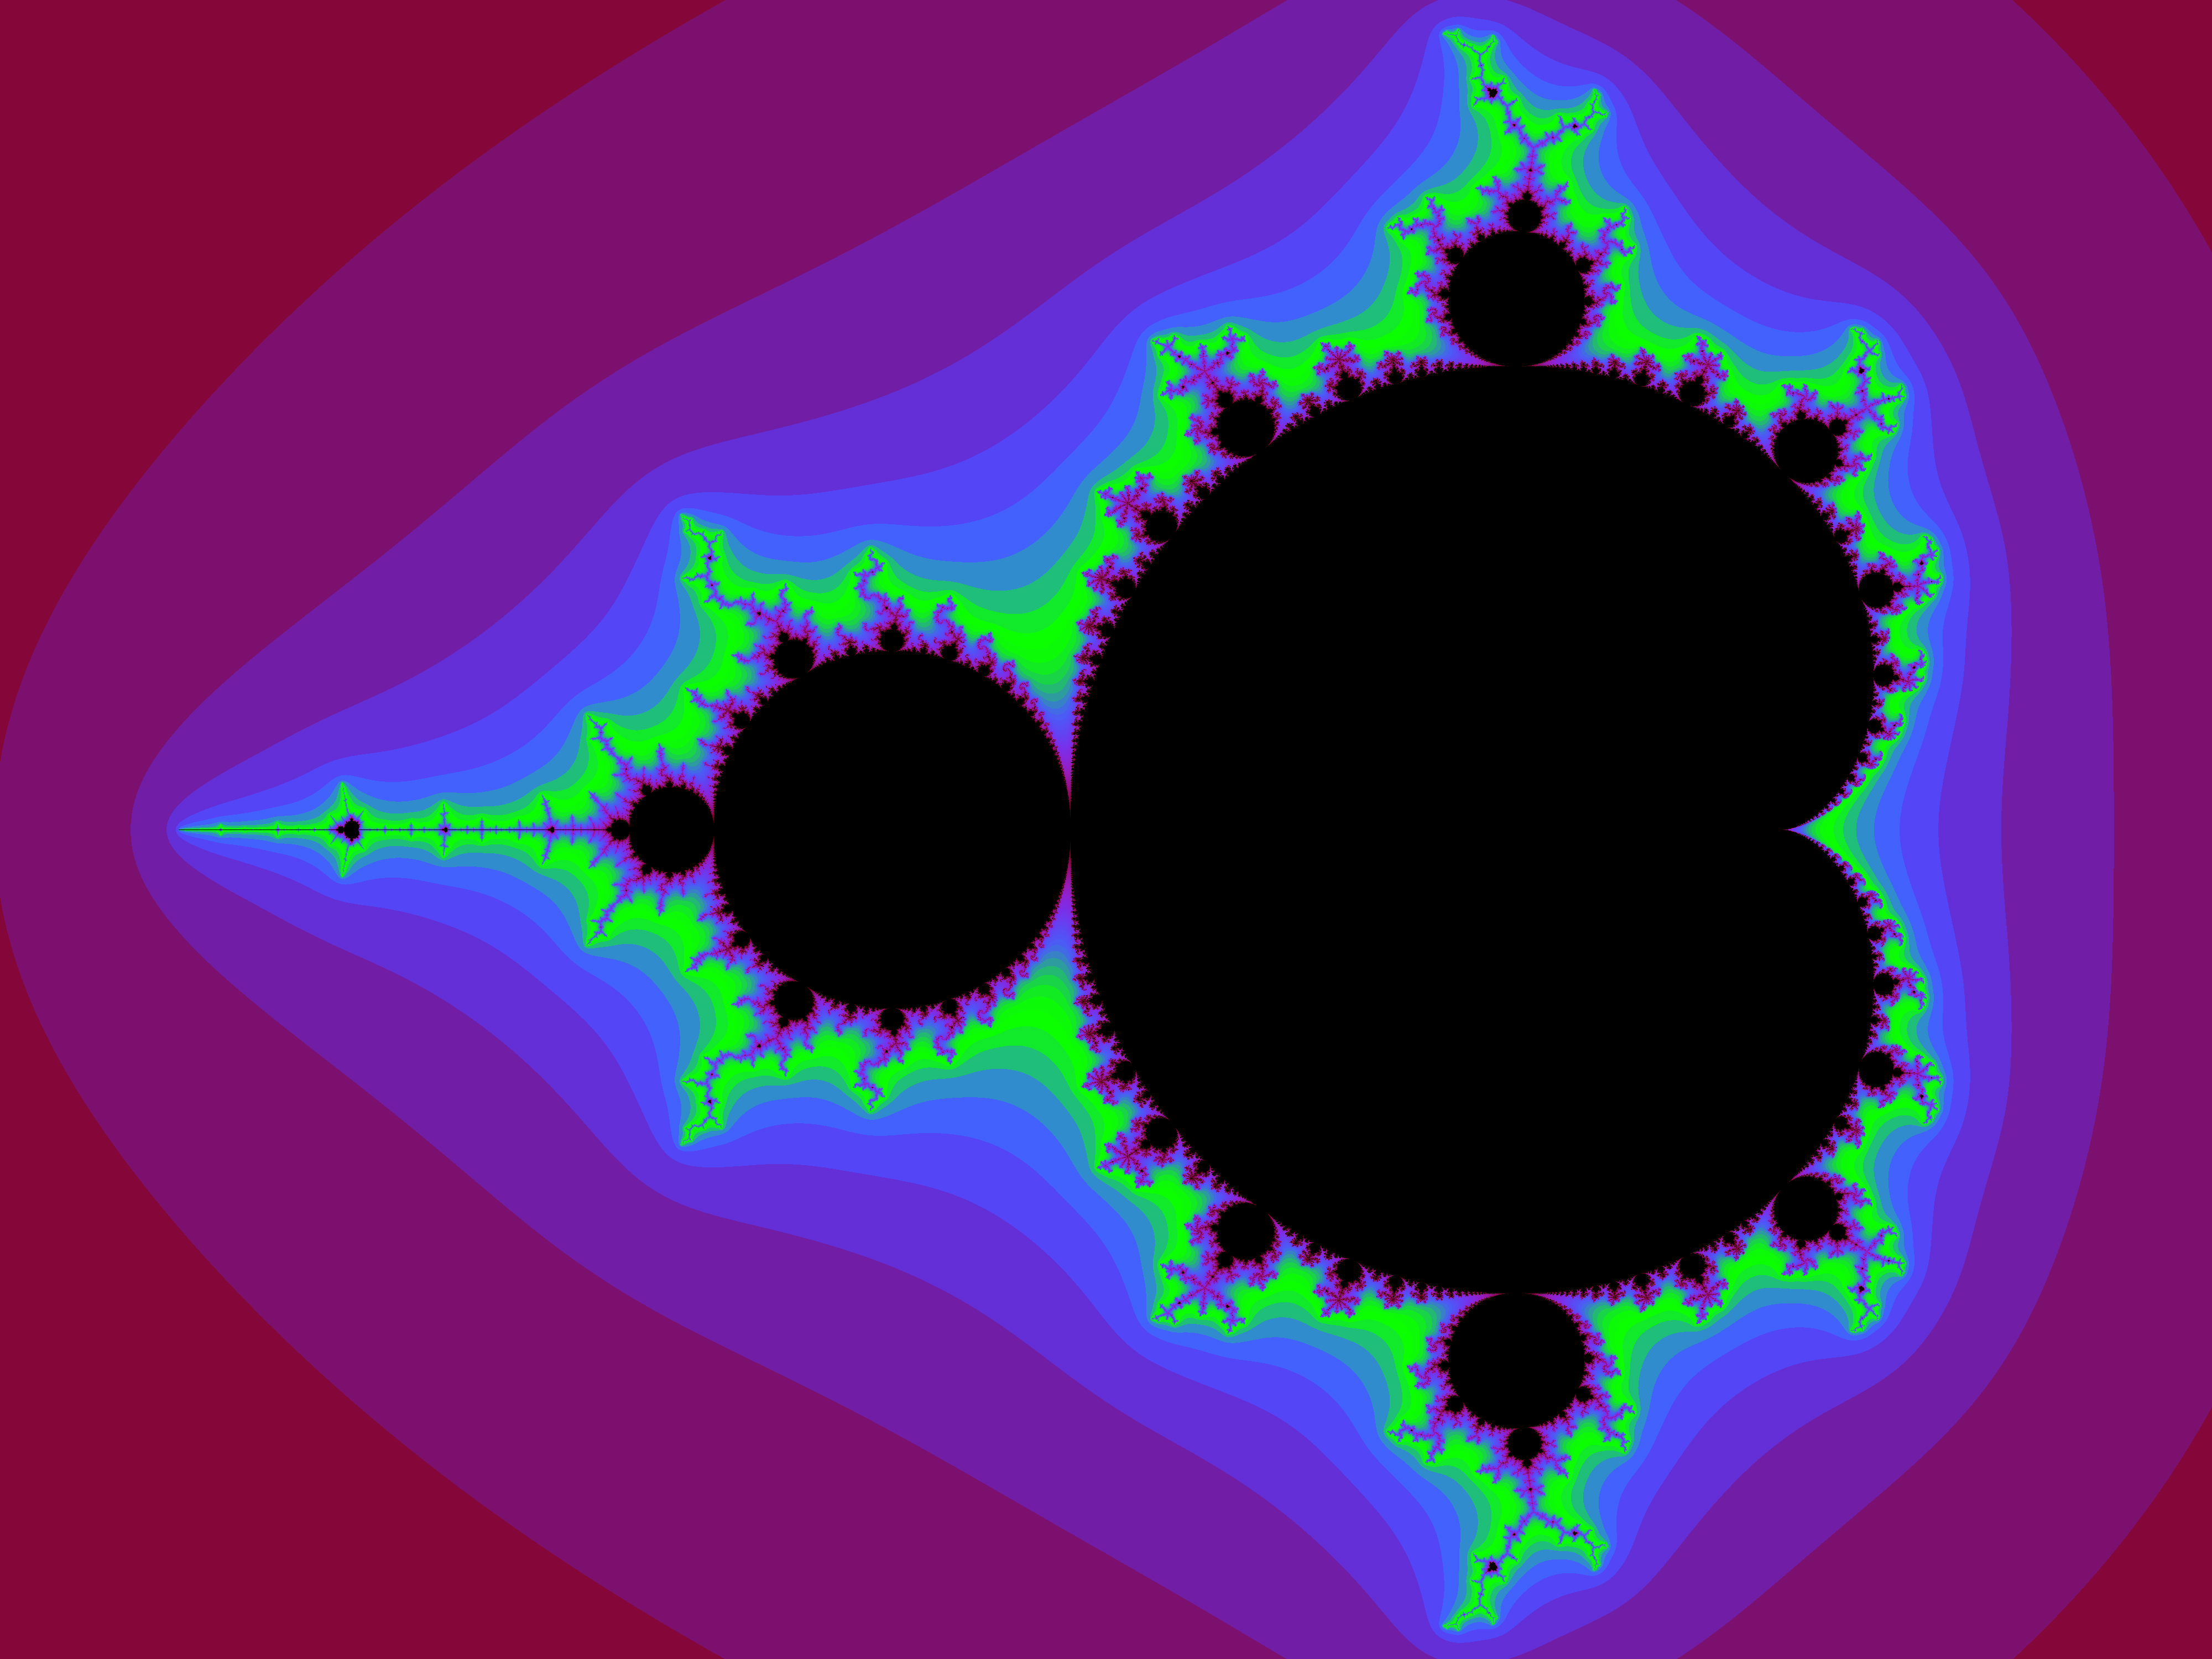
\includegraphics[width=.9\linewidth, angle =90 ]{figures/Mandelbrot}
	\caption{Mandelbrot. Ein künstliches Fraktal.~\cite{fractal_mandelbrot}}
	\label{fig:frac_math}
\end{subfigure}%
\end{figure}

\subsection{Newton Fraktale}
Diese Fraktale erscheinen sich, wenn man das Newton Verfahren für Auffinden der Wurzeln der nichtlinearen Gleichungen auf Komplexe Ebene einsetzt.
Genauer gesagt, soll man versuchen, die Wurzel für jeden Punkt des gesuchten Bildes durch Newton Verfahren zu finden.\\
Zum Beispiel nehmen wir die Funktion $f(x) = x^3 -1$. 
Diese Funktion hat drei Lösungen auf Komplexe Ebene: $1$, $-\sqrt[3]{-1}$ und $(-1)^{2/3}$. 
Die Näherungswerte in Koordinatenform sind $(1, 0)$, $(-0.5, 0.866)$ und $(-0.5, -0.866)$. 
Die Punkte des Bildes, die sich durch das Newton Verfahren zu entsprechenden Wurzeln annähern, werden entsprechend mit rot, blau und grün gefärbt.
Das Fraktal auf dem Bild~\ref{fig:output3_0} repräsentiert die gewählte Umgebung.
Die Ursachen der komischen Mischung werden in der Sektion~\ref{sec:analy} erläutert.
\begin{figure}[ht]   
	\centering
	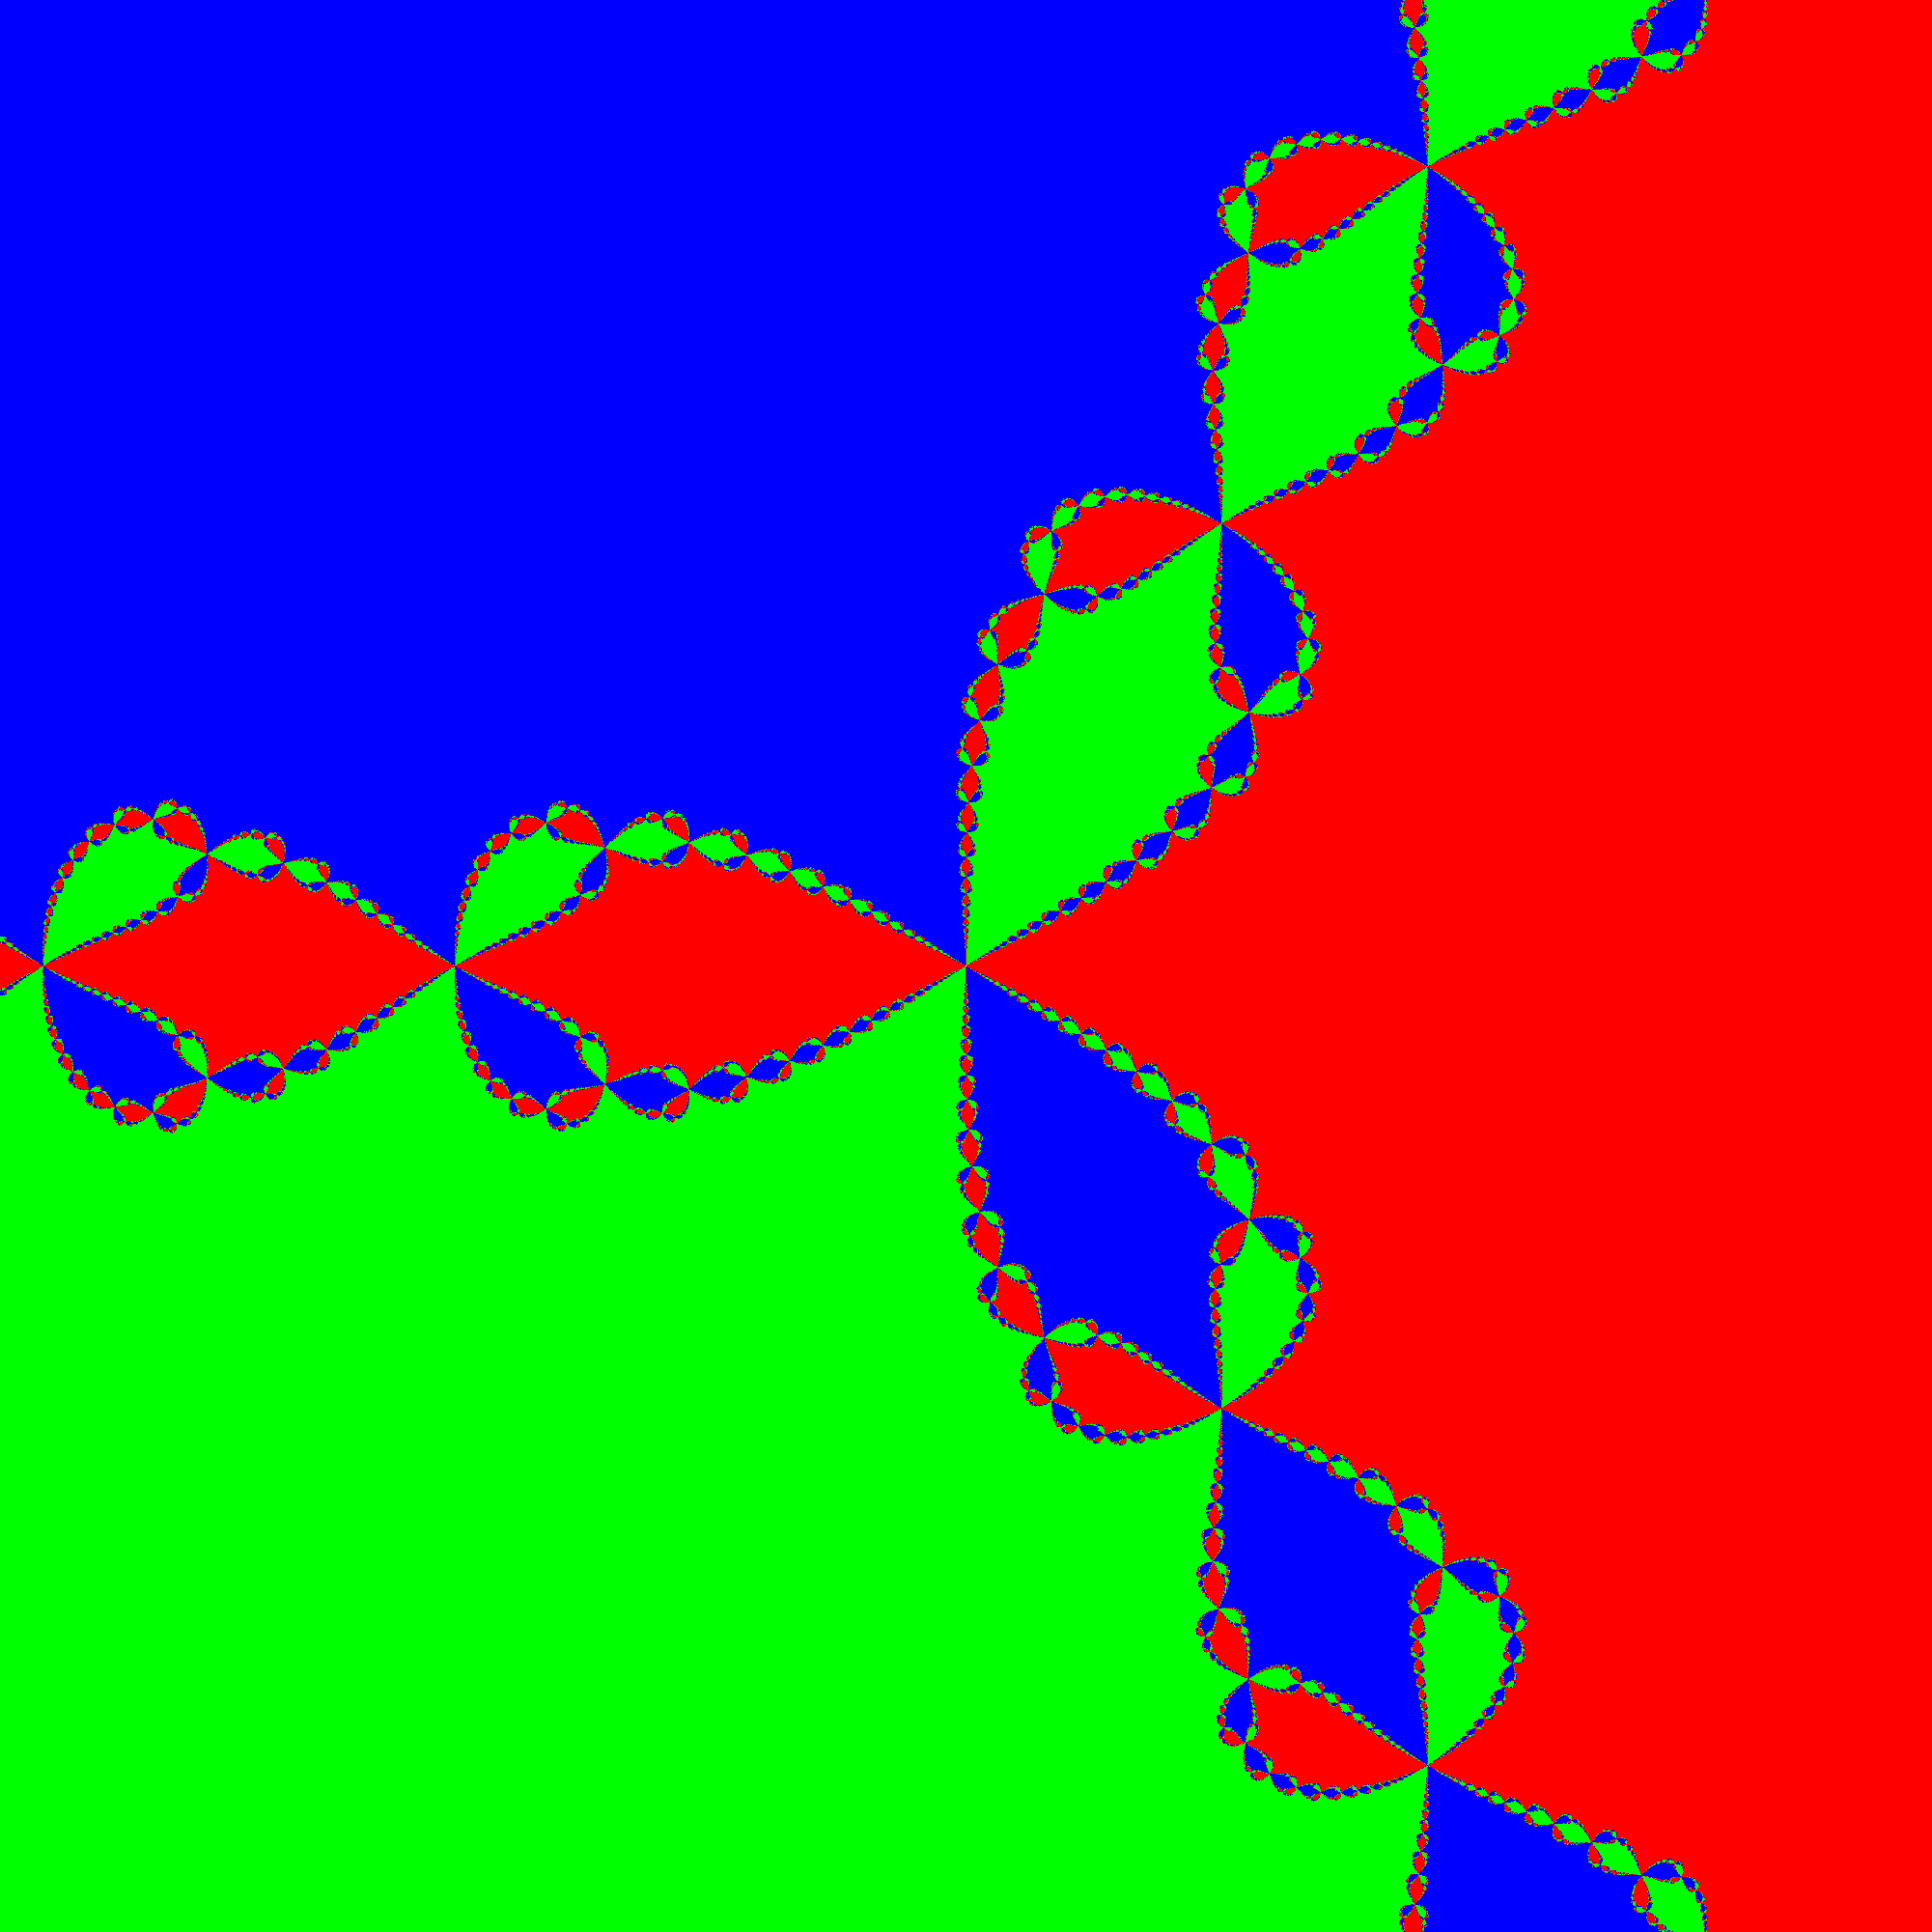
\includegraphics[width=.5\linewidth]{figures/output3_0}
	\caption{Newton Fraktal für $f(x)=x^3-1$ }
	\label{fig:output3_0}
\end{figure}

\section{Visualisierung}\label{sec:vis}
In diesem Abschnitt wird ein Programm entwickelt, das Bilder mit der Newton Fraktale generiert.
Außerdem wird es ein Beispiel vorgestellt, wie man Animationen erzeugen kann.

\subsection{Bildgenerierung}\label{subs:vis:bild}
Hier wird ein Programm beschreibt, die Newton Fraktale visualisiert.
Als Programmiersprache wurde Java gewählt.

\subsubsection{Bibliotheken}
Zusätzlich zu allgemeine Java-Bibliothek wurde noch das\\ $javax$.$imageio$.$ImageIO$ verwendet.
Das ist die öffentliche Bibliothek für die Arbeit mit Bildern, die, unter anderem, für das .$png$ Format geeignet ist.
Das PNG (Portable Network Graphics) Format passt für unsere Ziele ideal, wegen kleines Gewicht und keinen Qualitätsverlust der Dateien.

\subsubsection{Bild}
Mit Hilfe der $javax$.$imageio$.$ImageIO$ kann man sehr einfach die .$png$ Bildern erzeugen. 
Ein Beispiel ist in der Auflistung~\ref{lst:png}.
\begin{lstlisting}[float,caption=Ein Beispiel für die PNG Generierung, label=lst:png,captionpos=b]
BufferedImage bi = new BufferedImage(width, height, TYPE_INT_ARGB) ;
ImageIO.write(bi, "png", outputfilename);
\end{lstlisting}
Um den Bildinhalt einzusetzen, benutzt man den $bi.setRGB(x, y, Color);$ Befehl.\\
Natürlich soll man einen bestimmten Bereich des Fraktales wählen, um es zu zeichnen. 
Bei dem Programm wählt man den Startpunkt durch $X$ und $Y$ Koordinatenwerte, die Bildschirmgröße $Size$ und die Auflösung $resolution$. 

\subsubsection{Komplexe Zahlen}
Für die Bearbeitung der komplexen Zahlen ist eine neue Klasse implementiert, die die Arbeit mit komplexen Zahlen erleichtert. 
So kann man komplexe Zahlen addieren, abrechnen, multiplizieren, dividieren und potenzieren.

\subsubsection{Newton Verfahren}
Um Newton Verfahren zu benutzen, soll man manuell die Ableitung berechnen, die iterative Newton Funktion ausfinden und im Programmkode umwandeln.
Außerdem assoziiert man mit jeder Wurzel eine Farbe, um später das Bild zu zeichnen.
Als Beispiel nehmen wir die Funktion $f(z) = z^3 - 2z + 2$.
Die entsprechende Ableitung hat die Form $f'(z) = 3z^2 - 2$ und die iterative Funktion des Newton Verfahrens $z_{n+1} = \frac{2z_n^3 - 2}{3z_n^2 - 2}$.
Und hier steht der Programmkode für die iterative Funktion.
\[
	devide(mult(hoch(wert,3),2).add(-2), mult(hoch(wert,2),3).add(-2));
\]
Die Funktion wird iterativ für jedes Pixel des Bildes verwendet, um die Farbe zu berechnen.
Natürlich, man soll nach jedem Schritt Prüfen, ob die maximale Anzahl der Schritten $N$ nicht überschreitet wird und ob der Punkt schon die Wurzel ist. 
Das heißt, dass es für jeden gefundenen Punkt $z_n$ geprüft werden soll, ob $n > N$ oder $f|(z_n)| < \varepsilon$ ist.
Falls einer der beiden Fälle eintritt, bricht man die iterative Berechnung ab.
Im ersten Fall bezeichnet man das Punkt mit weiße Farbe, im zweiten - mit Farbe assoziierte mit der gefundenen Wurzel. 

\subsubsection{Lösungen} 
Da man manuell Farben für unterschiedliche Wurzeln wählen will, soll man alle Wurzeln mit assoziierten Farben im Programmkode eintragen. 
Ein Beispiel für die Funktion $z^3 - 1$ findet man in der Auflistung~\ref{lst:punkt}. 
Jede Wurzel wird durch zwei Zahlen festgestellt, die reale und imaginäre Parts abbilden.
Letzte drei Argumente definieren die Farbe der Wurzel in das RGB Format.
\begin{lstlisting}[caption=Wurzeln mit Farben für $z^3 - 1$, label=lst:punkt]
points.add(new point(1,	   0,	   255, 0,   0));
points.add(new point(-0.5, 0.866,  0,   255, 0));
points.add(new point(-0.5, -0.866, 0,   0,   255));
\end{lstlisting}

\subsubsection{Schatten}
Für bessere Informationswiedergabe darf man optional die Schatten einschalten.
Dann je mehr Schritten des Newton Verfahren nötig sind, desto dunkler das Pixel wird.  

\subsubsection{Programmkode}
Vollständige Programmkode kann man unter~\cite{source} finden.

\subsection{Animation}\label{subs:vis:anime}
Einer der einfachsten Wegen für die Animationserzeugung wurde gewählt. 
Das Programm wurde so geändert, dass $size$ und $outputfilename$ variabel werden. 
Dann im Zyklus wird eine Reihenfolge der Bildern generiert, so dass das neue Bild die Annäherung des Altes wird.
Die Animation wird aus diese Reihenfolge der Bildern mit Hilfe des~\cite{animegen} generiert.

\section{Analyse}\label{sec:analy}
Manche Newton Fraktale werden vorgestellt und analysiert.

\subsection{$z^3 - 1 = 0$}
Wie oben schon gesagt war, hat diese Gleichung drei Lösungen auf Komplexe Ebene: $+1$, $-\sqrt[3]{-1}$ und $(-1)^{2/3}$. Entsprechende Newton Fraktal ist auf dem Bild~\ref{fig:output3_0} visualisiert. 

\begin{figure}[ht]   
	\begin{subfigure}{.5\textwidth}
		\centering
		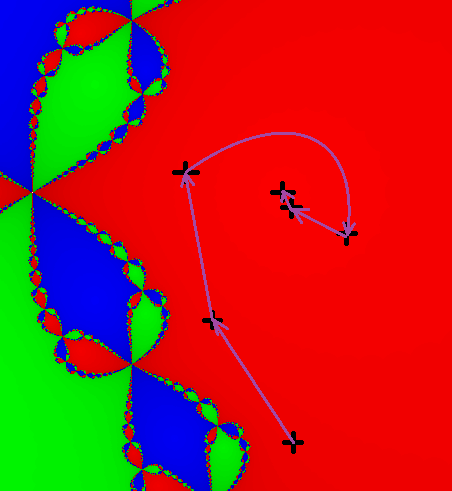
\includegraphics[width=.7\linewidth]{figures/output_points3}
		\captionsetup{width=0.8\textwidth}
		\caption{Die Konvergenz des Punktes (1, 1) für $f(z)=z^3-1$ }
		\label{fig:output_points3}
	\end{subfigure}%
	\begin{subfigure}{.5\textwidth}
		\centering
		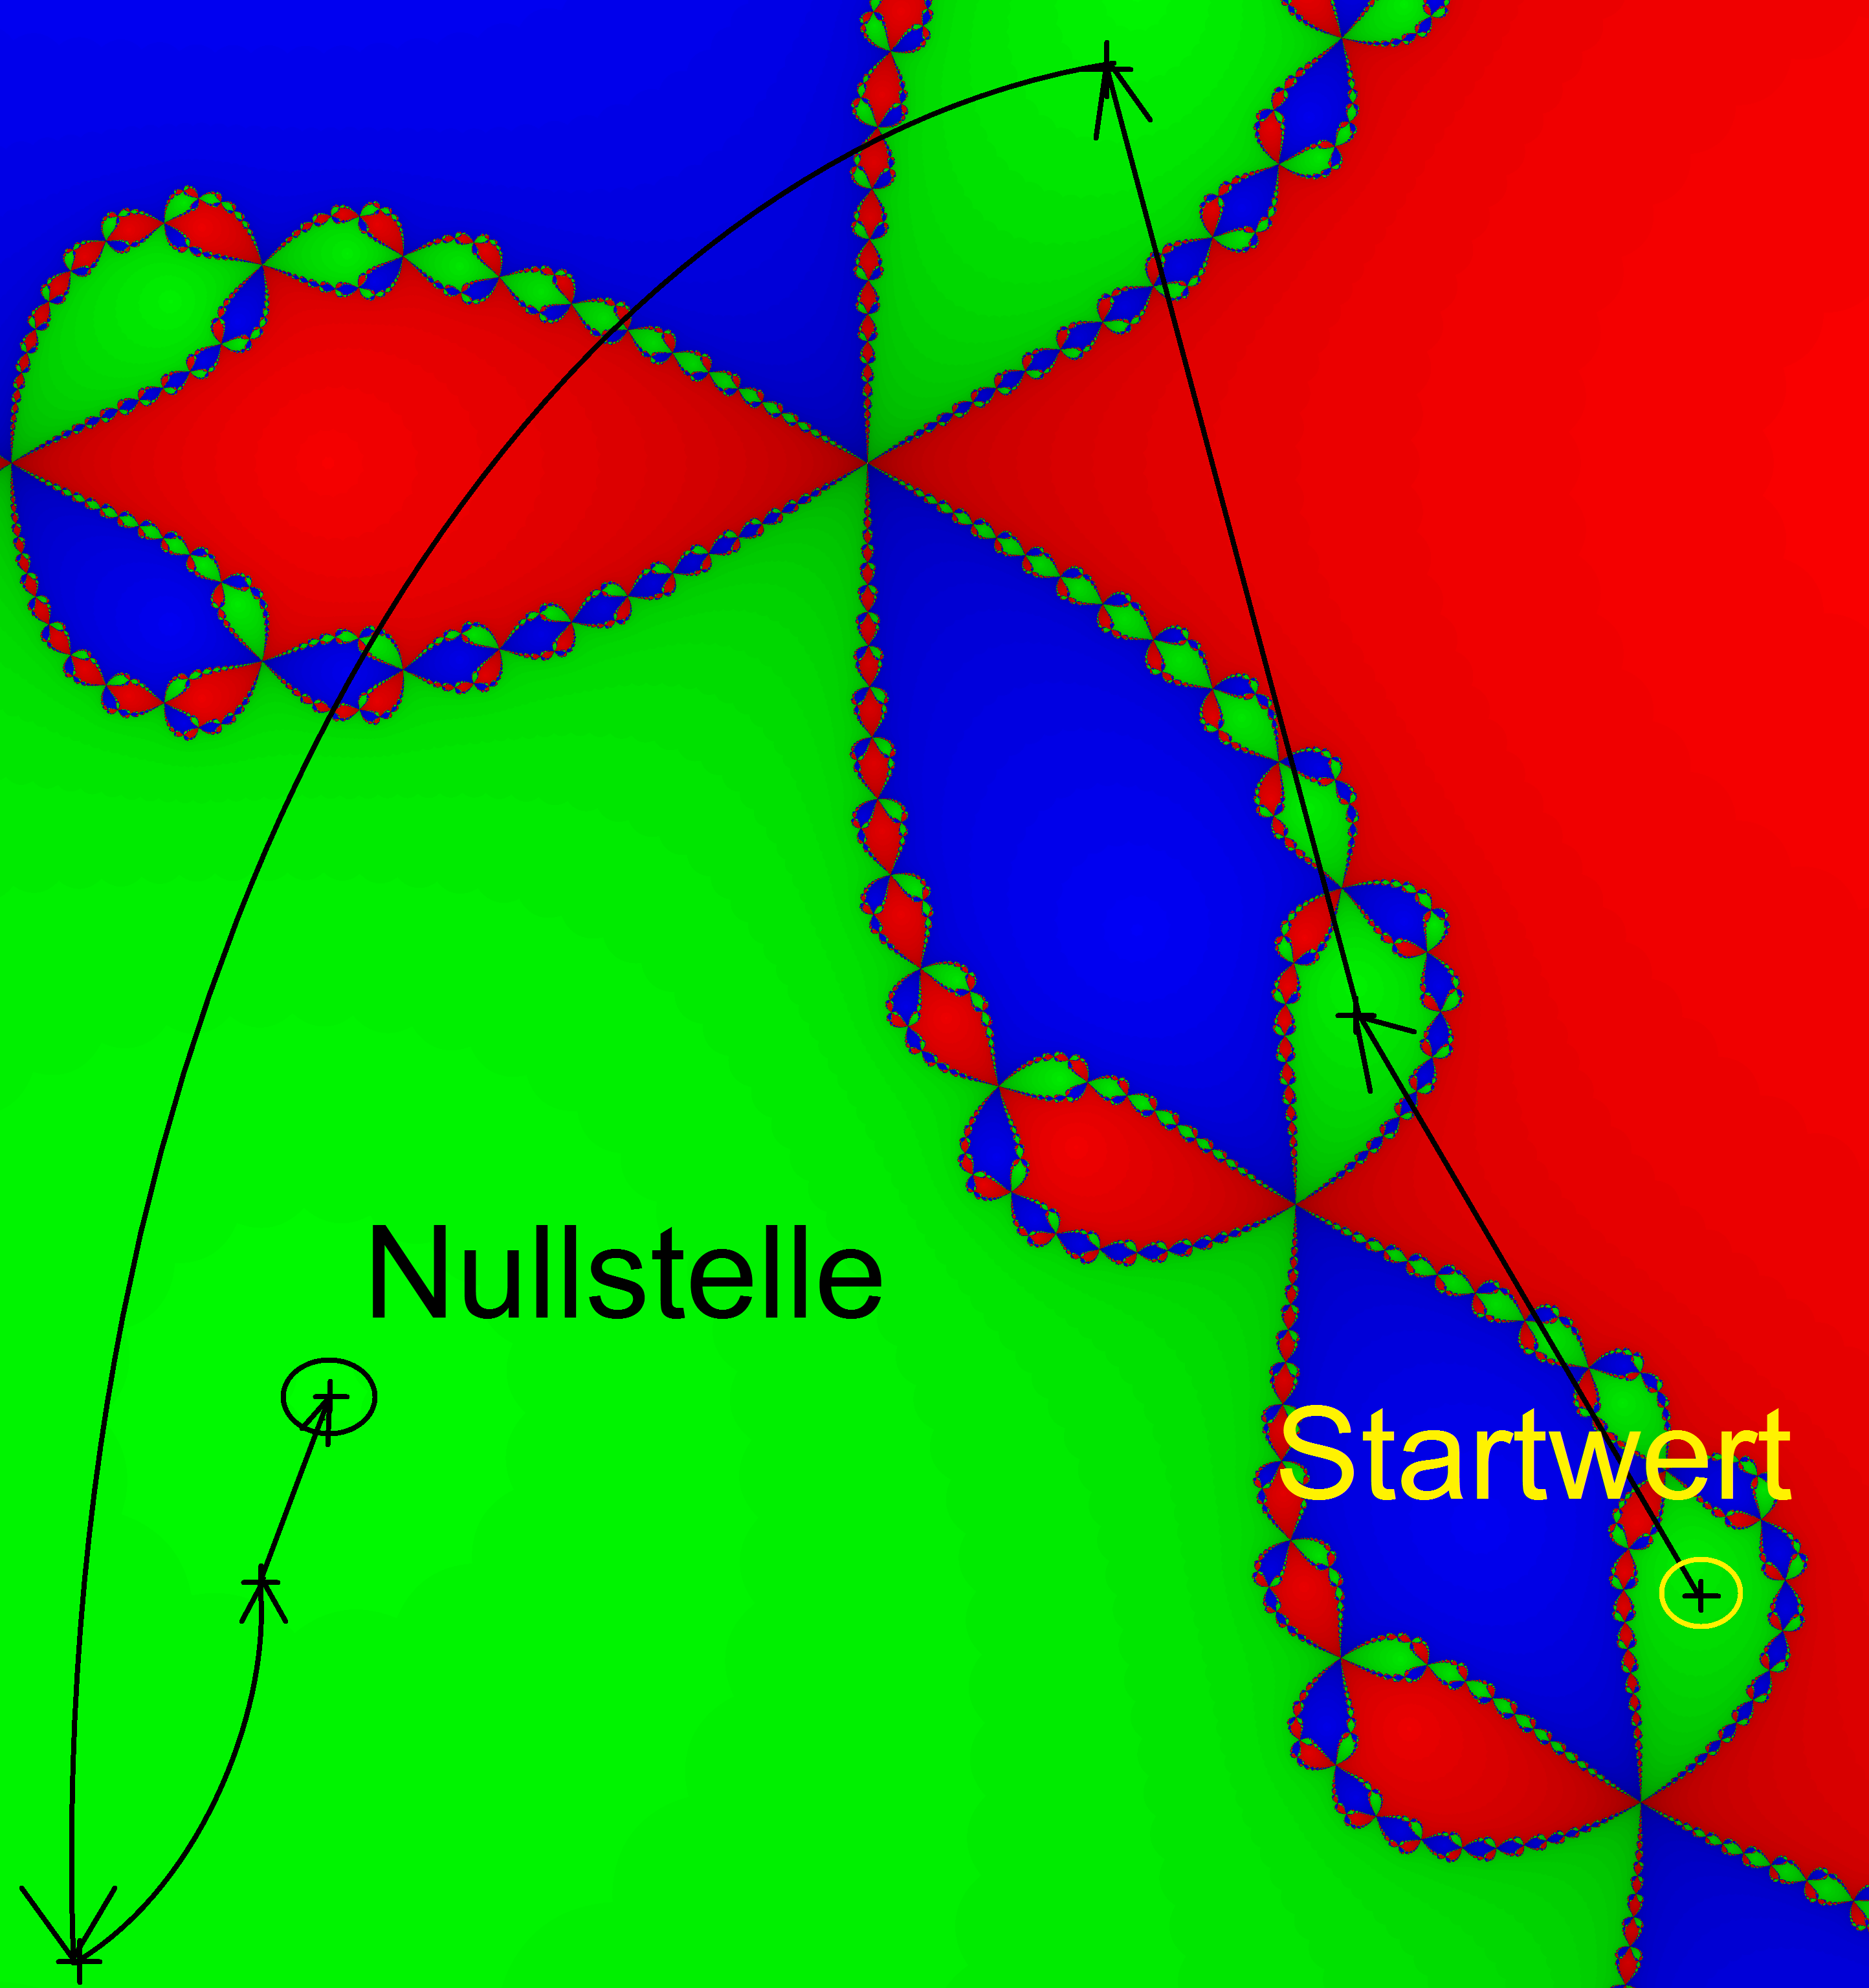
\includegraphics[width=.7\linewidth]{figures/output_points_g3}
		\captionsetup{width=0.8\textwidth}
		\caption{Die Konvergenz des Punktes (0.9, 1) für $f(z)=z^3-1$ }
		\label{fig:output_points_g3}
	\end{subfigure}%
\end{figure}
Wenn man versucht die Grenze zwischen zwei Zonen zu annähern, sieht man, dass dort immer dritte Zone vorkommt. 
Das wiederholt sich rekursiv bei Annäherung.
In anderen Worten, wenn man einen Anfangspunkts $z_0$ wählt, der gegen $+1$ konvergiert und einen Punkt $z_1$, der gegen  $-\sqrt[3]{-1}$ konvergiert, dann existiert es zwischen $z_0$ und $z_1$ immer einen dritten Punkt $z_2$, der noch näher zu $z_0$ als $z_1$ liegt und zu $(-1)^{2/3}$ konvergiert. \\
Wichtigste Frage ist: warum sehen die Zonen nicht wie die einfachen 120-Grad-Sektoren aus?
Anfang letztes Jahrhunderts gelang es zwei französischen Mathematiker Gaston Julia und Pierre Fatou zu zeigen, dass die Grenzpunkten eines Einzugsgebiets die Grenzpunkte aller Einzugsgebiete sind. 
Folglich können Iterationen mit mehr als zwei Einzugsgebieten keine einfach zusammenhängenden Liniensegmente als Gebietsgrenzen in 2D haben. 
Solche Grenzen müssen zwangsläufig fraktalen Natur sein, bestehend aus vollständig separaten Punktmengen - sozusagen eine unendlich feine Staubwolke aus nichtabzählbar vielen Staubpartikelchen.~\cite{frak_cha}
Machen wir uns damit ein bisschen vertraut, indem wir die Nullstelle (der Punkt $0:0$) anschauen.
Logischerweise soll die Nullstelle zwischen allen Zonen liegen.
Die Null selbst konvergiert überhaupt nicht, da die Einsetzung $z=0$ zu Division durch Null bei Newton Verfahren folgt.
Aber diese Nullstelle ist nicht allein, außer es existieren noch unendlich viele Punkte, die gegen die Nullstelle konvergieren und für die auch gilt, dass daneben alle Zonen vorhanden sind.
(Das folgt aus der lineare Natur des Newton Verfahrens.)
Diese Punkten, die gegen die Null konvergieren, bilden diese komische Grenze Zwischen den Zonen.\\
Zum Beispiel betrachten wir die Punkte (1, 1) und (0.9, 1). 
Die Konvergenz des Punktes (1, 1) wird auf dem Bild~\ref{fig:output_points3} vorgestellt.\\
Der Punkt liegt weit genug von der Grenze und wird eindeutig konvergiert, trotzdem sieht man so ein Sprung, die sehr oft bei Newton Verfahren eintreten können.\\
Jetzt betrachten wir das Punkt (0.9, 1) auf dem Bild~\ref{fig:output_points_g3}.
Die Konvergenz des Punktes zeigt eindeutig, wie die iterative Schritte des Newton Verfahrens funktionieren und wie man zu solchen Bildern kommt. 
Erste zwei iterative Schritte behalten sich gleich wie bei dem Punkt (1, 1), was die lineare Natur des Newton Verfahrens bekräftigt. 
Aber dann, neben der Nullstelle, wird es nach grünen Gebiet geworfen.
Die Punkten neben Grenzen bewegen sich zuerst in die Richtung der Nullstelle und dann rasant in die passende Zone springen.\\
Zusätzliches Beispiel wird auf dem Bild~\ref{fig:output3_3} vorgestellt, wo die helle Bereiche die am schnellsten konvergierende Punkte bezeichnen.
\begin{figure}[ht]   
	\begin{subfigure}{.5\textwidth}
	\centering
		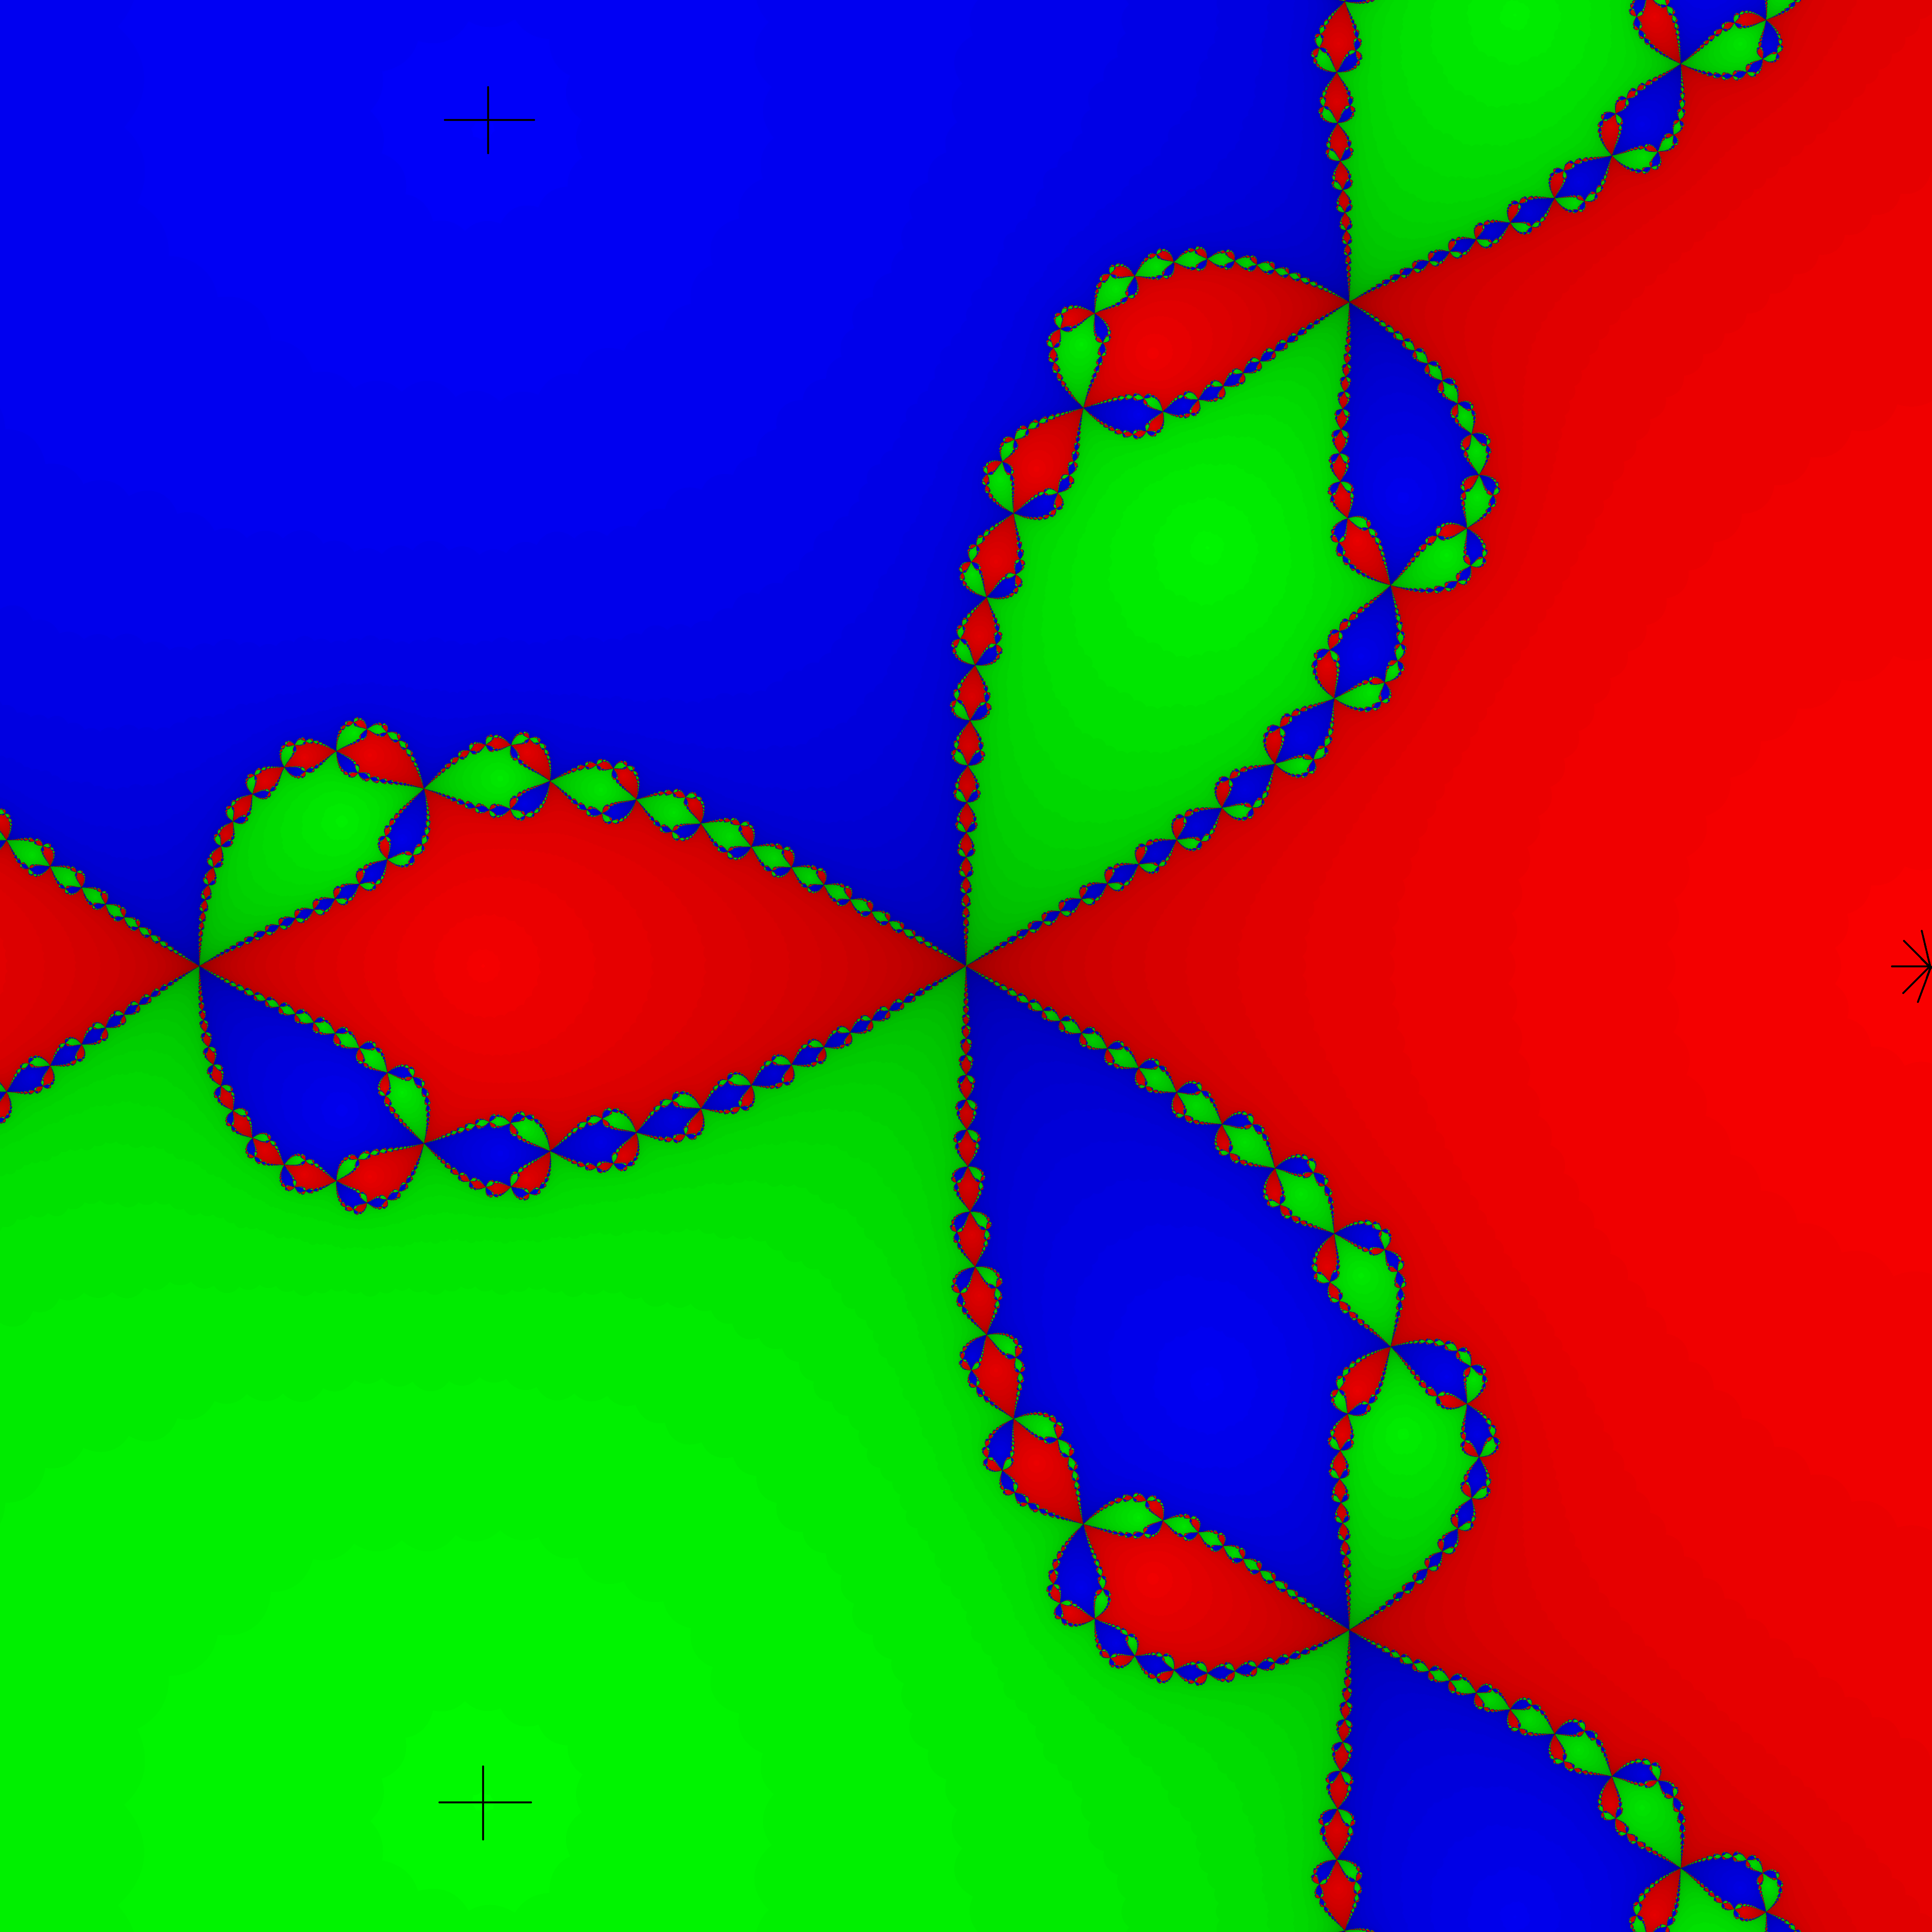
\includegraphics[width=.7\linewidth]{figures/output3_3}
		\captionsetup{width=0.8\textwidth}
		\caption{Die Konvergenzgeschwindigkeit durch die Helligkeit für $f(z)=z^3-1$ }
		\label{fig:output3_3}
	\end{subfigure}%
	\begin{subfigure}{.5\textwidth}
	\centering
		\includegraphics[width=.7\linewidth]{figures/output5_3}
		\captionsetup{width=0.8\textwidth}
		\caption{Das Newton Fraktal für $f(z)=z^5-1$ }
		\label{fig:output5_3}
	\end{subfigure}%
\end{figure}

\subsection{$z^5 -1 = 0$}
Das Bild~\ref{fig:output5_3} illustriert das entsprechende Newton Fraktal. 
Der einziger Unterschied liegt in der Anzahl der Zonen und Lösungen.
Wie bei $z^3 -1 = 0$ sind die Grenzpunkten eines Einzugsgebiets die Grenzpunkte aller Einzugsgebiete, was für die fünf Zonen interessanter aussieht.

\subsection{$z^5 + (5+2i)z^3 - 2-i $}
Das entsprechende Newton Fraktal (das Bild~\ref{fig:output_f7}) besitzt eine interessante Struktur. 
Der Grund dazu liegt in der Position der Wurzeln.
Die Nullstelle, die grüne und die rote Zonen liegen fast auf die Gerade.
Das Gleiche gilt für die Nullstelle, die blaue und die hellblaue Zonen.
Unabhängig davon, dass die hellblaue und die grüne Zonen weit weg von der Nullstelle liegen und mit der roten und blauen Zonen abgegrenzt sind, konvergieren manche Punkte neben der Nullstelle gegen das Grün und das Hellblau.
\begin{figure}[ht]   
	\begin{subfigure}{.5\textwidth}
		\centering
		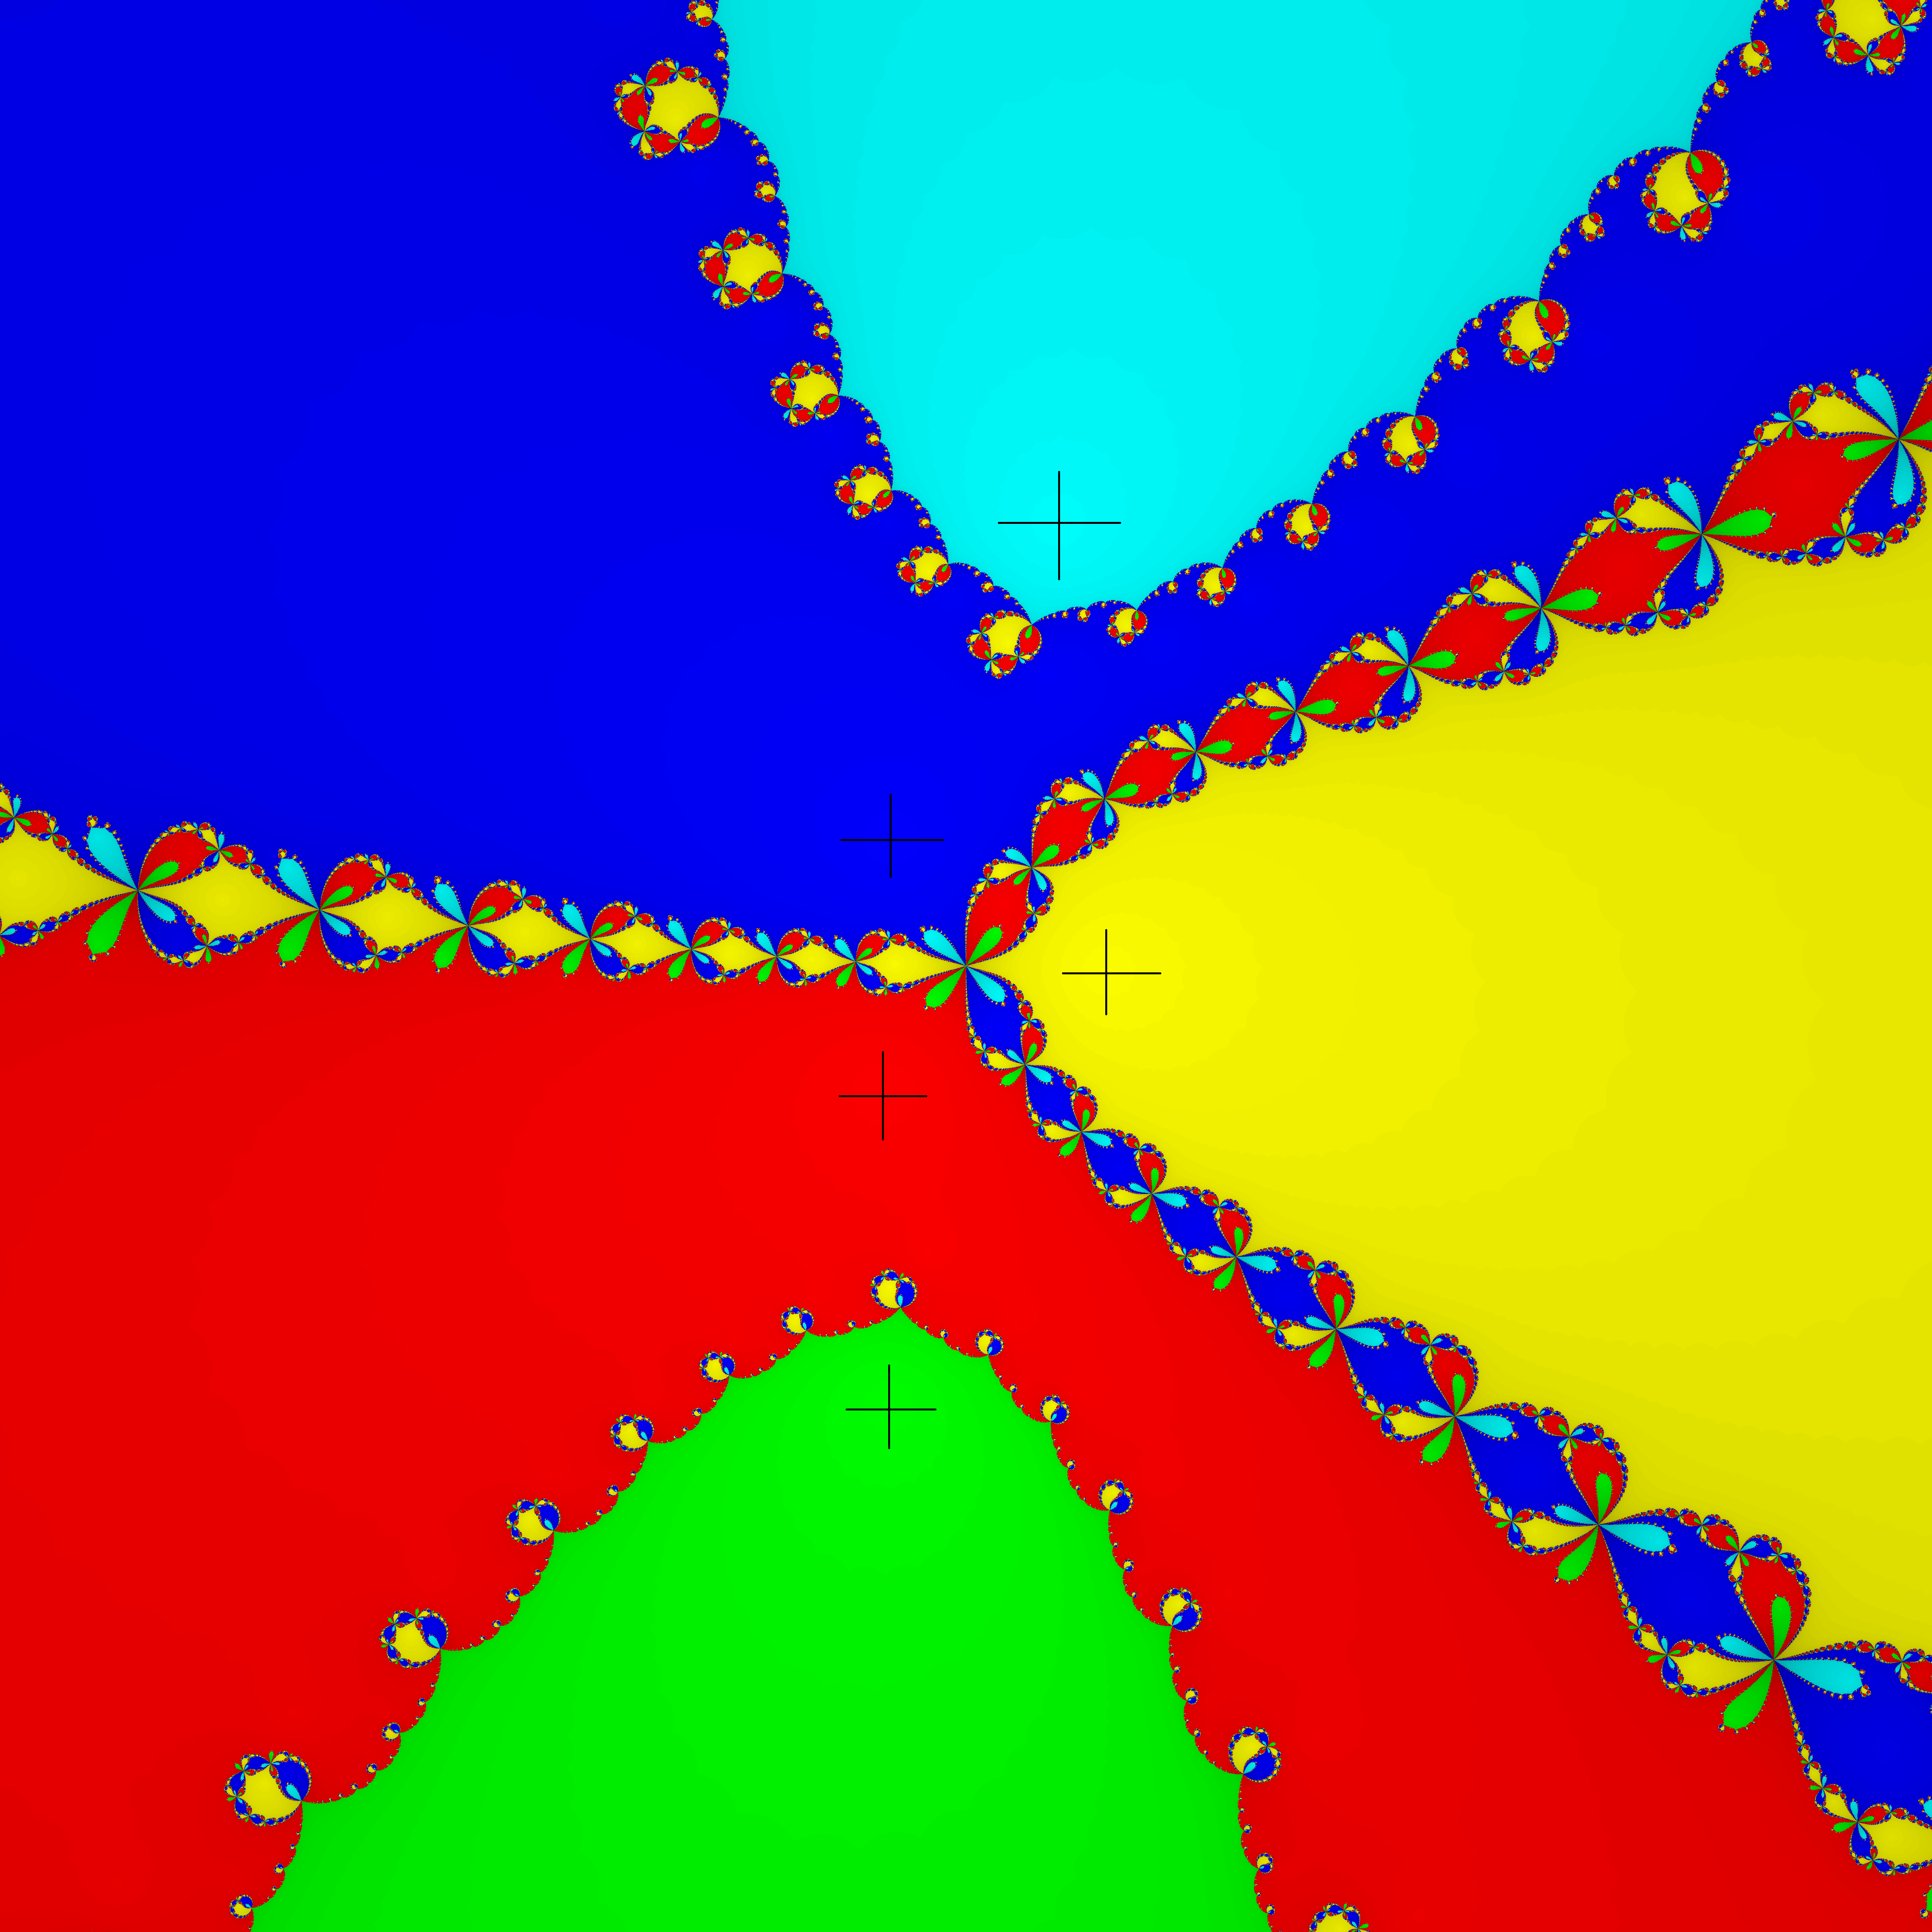
\includegraphics[width=.7\linewidth]{figures/output_f7}
		\captionsetup{width=0.8\textwidth}
		\caption{Das Newton Fraktal für $f(z)=z^5 + (5+2i)z^3 - 2-i $ }
		\label{fig:output_f7}
	\end{subfigure}%
	\begin{subfigure}{.5\textwidth}
		\centering
		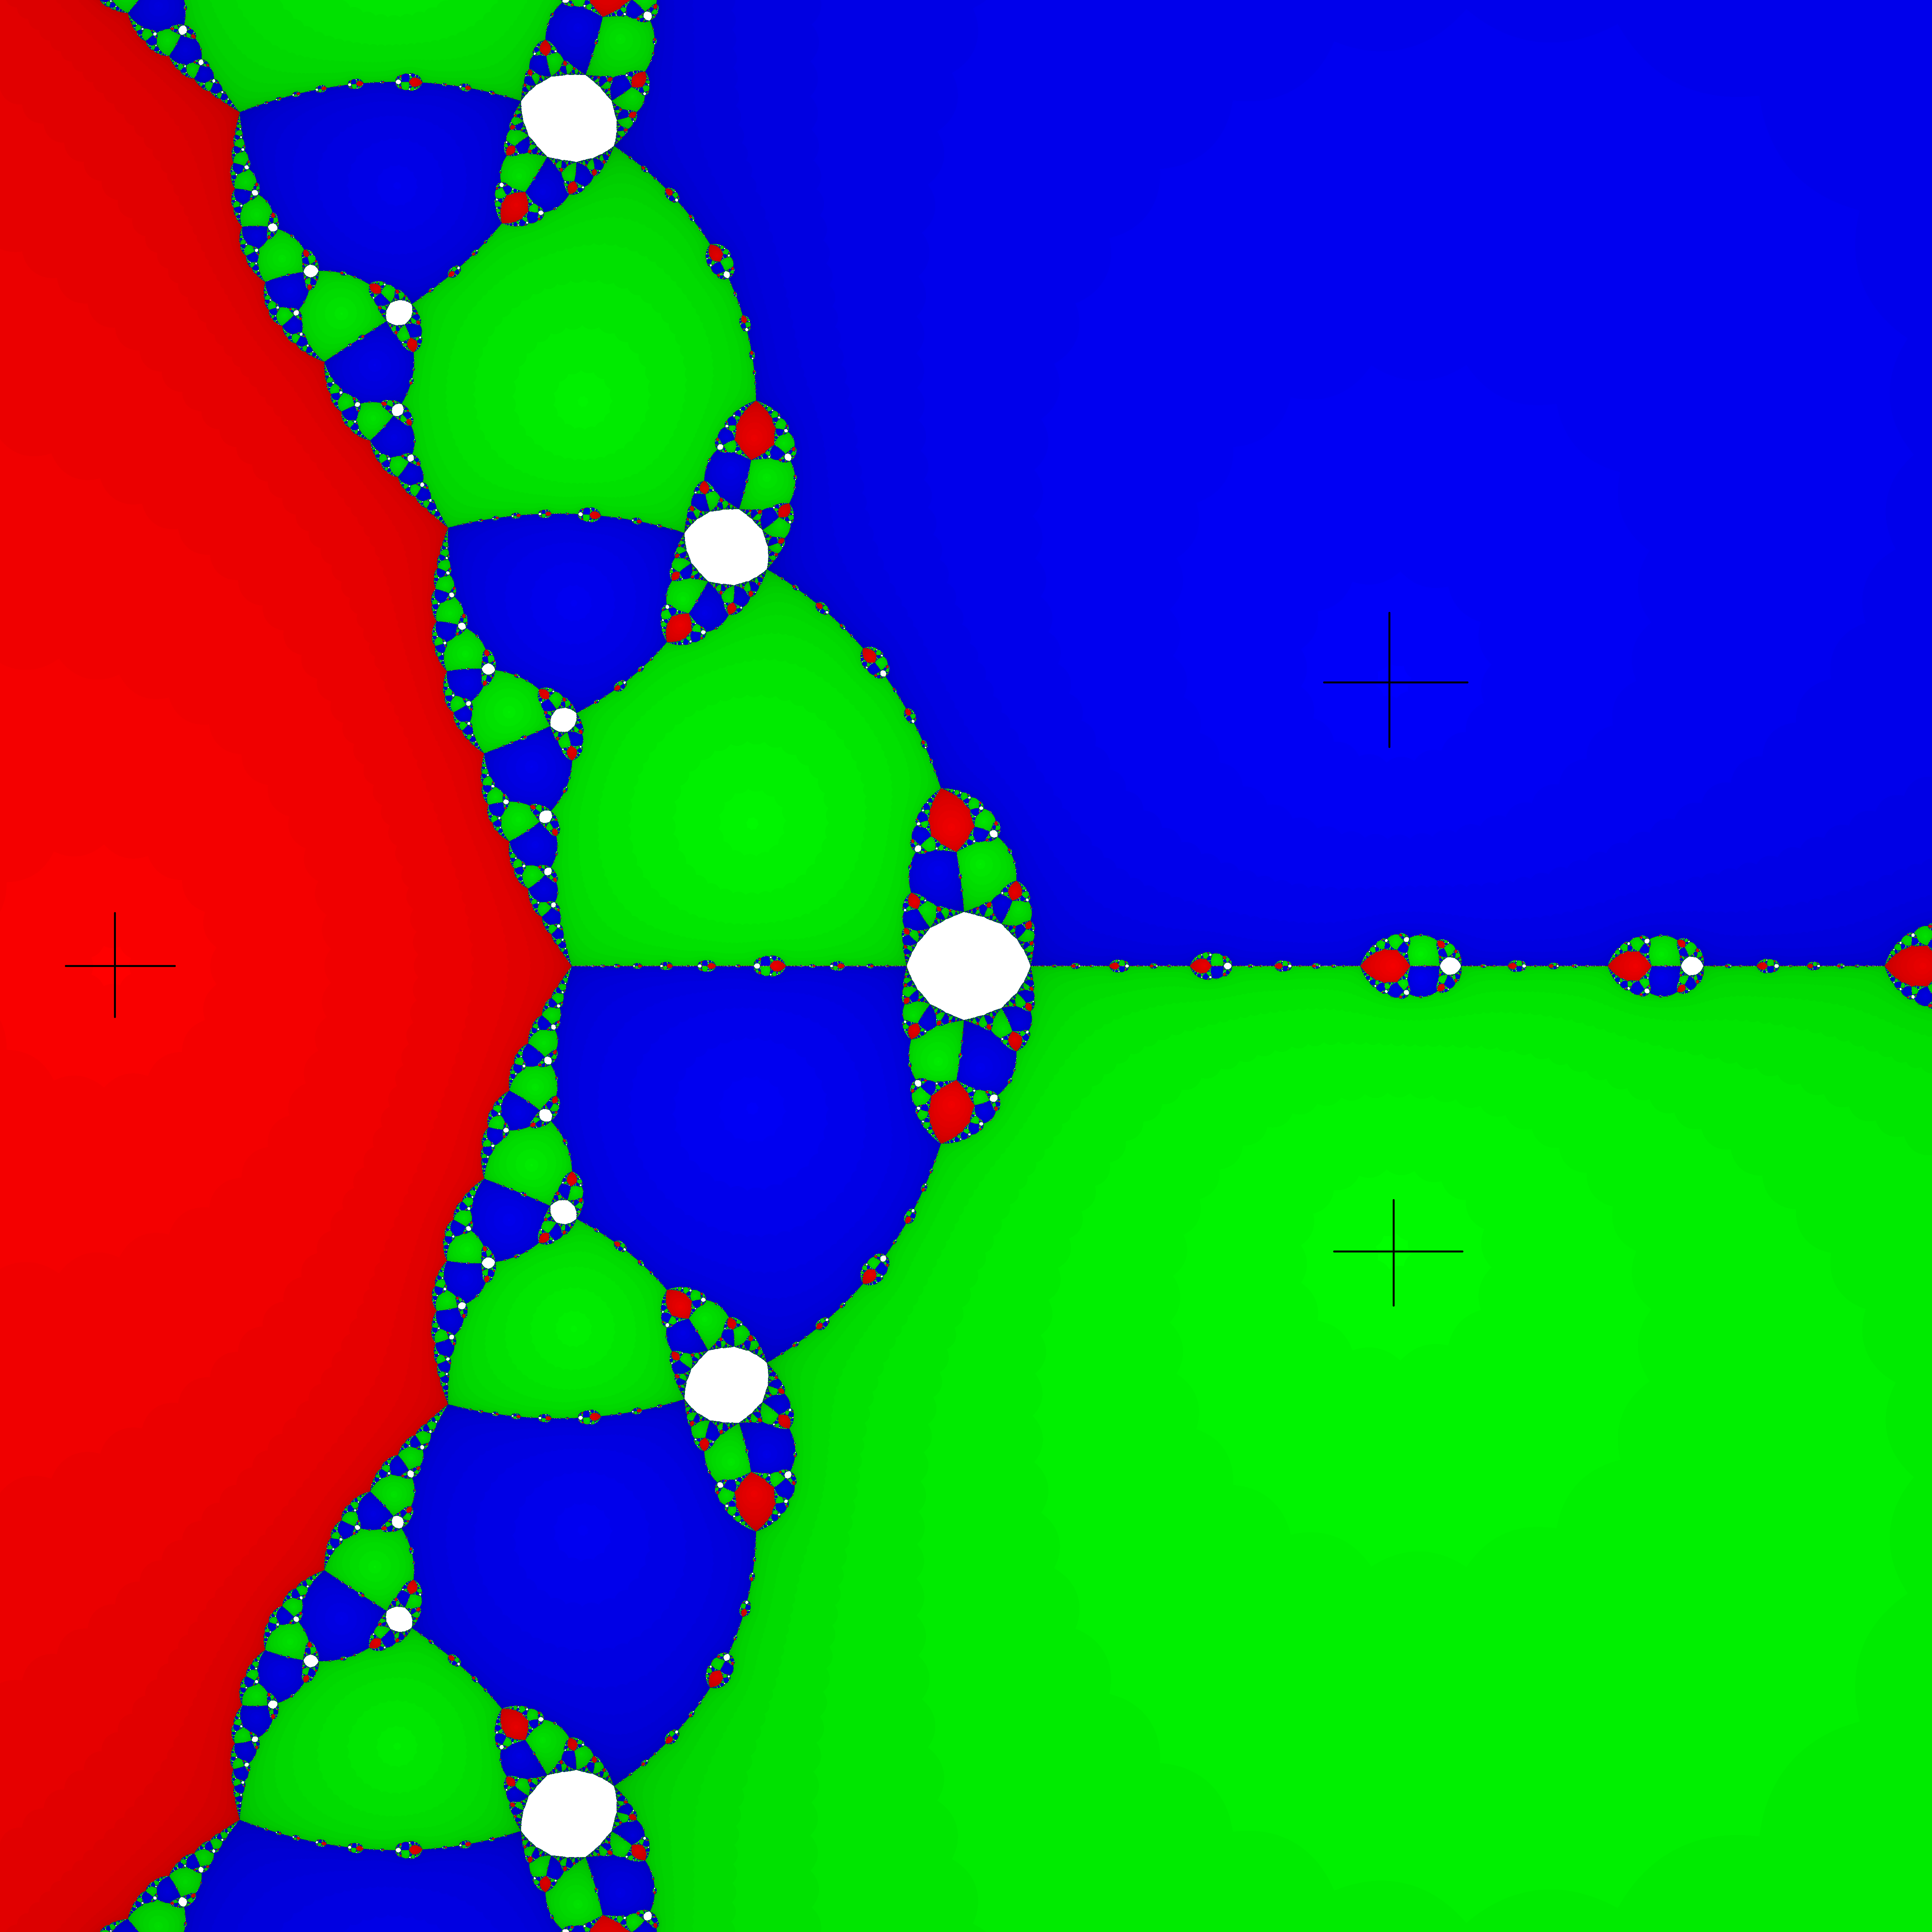
\includegraphics[width=.7\linewidth]{figures/output_f5}
		\captionsetup{width=0.8\textwidth}
		\caption{Das Newton Fraktal für $f(z)=z^3 - 2z + 2$ }
		\label{fig:output_f5}

	\end{subfigure}%
\end{figure}

\subsection{$z^3 - 2z + 2$}
Das Bild~\ref{fig:output_f5} illustriert das Newton Fraktal für diese Funktion.
Wie man sieht, hier gibt es ziemlich große weiße Bereiche. 
Was passiert dort?
Um diese frage zu beantworten, sollen wir ein paar Schritte des Newton Verfahrens manuell ausführen.
Die iterative Funktion hat die folgende Form:
\[
z_{n+1} = \frac{2z_n^3-2}{3z_n^2-2}
\]
Probieren wir das Punkt (0,0), oder $z_0 = 0$ ist.
Nach der Einsetzung in die iterative Formel bekommt man $z_1 = 1$.
Sieht noch gut aus, aber was passiert weiter?
Erstaunlicherweise ist $z_2$ wieder gleich $0$.
So springt der Wert zwischen $0$ und $1$, was ein gutes Beispiel ist, warum man die Anzahl der Schritten begrenzen soll.
Aber was passiert neben dem Punkt (0,0), sodass diese weiße Gebiete so groß sind?
Iterieren wir der Punkt (0.1, 0), der ziemlich nah zu der Nullstelle liegt.
Dann ist $z_0=0.1$; $z_1= 1.014213$ und $z_2= 0.079655$.
Man sieht, dass $z_2$ noch näher zu der Nullstelle liegt, als $z_0$.
Je mehr iterative Schritte man ausführt, desto näher es zu der Nullstelle hintritt.
Wenn man andere Punkte aus der Umgebung der Nullstelle zu iterieren versucht, werden die Punkten, die nah genug liegen, gegen die Nullstelle konvergieren.
So werden die weißen Fällen gebildet, die diese Funktion auszeichnen.

\section{Zusammenfassung}
Numerische Lösungen von nichtlinearen Gleichungen durch Approximation sind in der modernen Welt überall gebraucht.
Die approximative Berechnungen bringen viele unerwartete Probleme und interessante Ereignisse.
Newton Fraktale ist eine der Ereignisse. 
Die Erforschung des Phänomens ist wichtig für unsere Verständnis des Newton Verfahrens.\\
Im Rahmen dieser Arbeit sind theoretische Grundlagen vorgestellt, wichtigste Begriffe erläutert und erklärt.
Dann hat man die Software entwickelt, die Newton Fraktale visualisiert.
Es ist eine Methode vorgestellt, die beschreibt, wie man Animationen erzeugen kann.
Danach sind manche Newton Fraktale analysiert und die Ursachen für ihre interessante Struktur vorgestellt.
% Literaturverzeichnis ------------------------------------------------
\newpage
\bibliographystyle{alphadinLinkLocal}
\bibliography{literatur} 

%\iffalse
\end{document}
%\fi
